% !TEX root = ../main.tex
\chapter{Туршилт ба UI дүрслэл}\label{ch:ui}

\section{Зарчим}
Animation-ийн гол зарчим нь дэлгэц дээрх алхам бүр бодит thread-ийн хийсэн үйлдэл байх явдал юм. Хөтөч
эрэмбэлэлтийг өөрөө тооцоолдоггүй. Java дээрх thread-үүдийн бүртгэсэн event-үүдийг хүлээн авч дүрсэлнэ. Event
бүрт thread-ийн нэр ба \code{System.nanoTime}-аар хэмжсэн хугацаа байдаг тул хоёр sorter-ийн алхмууд хэрхэн
холилдсон, merger хэзээ эхэлснийг бодитоор нь харуулна. \code{./run.sh --web} ажиллуулаад \url{http://localhost:8080}
хаягийг нээнэ.

\section{Өөрчилж турших параметр ба удирдлага}
Хэрэглэгч тоонуудаа гараар оруулах эсвэл санамсаргүй жагсаалт үүсгэнэ ($n$, seed, min, max, хэлбэр: random,
sorted, reversed, duplicates). Sorter-L ба Sorter-R-д таван алгоритмаас тус тусад нь сонгоно. Удирдлага нь
Ажиллуулах, Тоглуулах / Түр зогсоох (\code{Space}), Алхам урагш (\code{→}) ба хойш (\code{←}), Эхнээс нь,
хурд (1--5000 алхам/сек), байрлалын гулсуур гэсэн товчнуудтай.

\section{Юуг ажиглах}
Дэлгэц эх массив \code{list[]}, хоёр дахь массив \code{result[]}, thread-үүдийн хугацааны шугам, thread бүрийн
карт (нэр, \code{tid}, төлөв, үйлдлийн тоо), сүүлийн event-үүд, үр дүн гэсэн хэсгүүдтэй (Зураг~\ref{fig:ui}).
\textcolor{cleft}{Цэнхэр} нь Sorter-L-ийн хэсэг, \textcolor{cright}{улбар шар} нь Sorter-R-ийн хэсэг,
\textcolor{cmerge}{ногоон} нь merger-ийн бичсэн утга, \textcolor{ccmp}{ягаан улаан} нь харьцуулж буй элемент,
цагаан нь сольсон элемент, бараан саарал нь merger аль хэдийн авсан элемент. Босоо зураас хуваалтын цэг \code{mid}-ийг заана.

\begin{figure}[H]
\centering
\begin{subfigure}{0.49\linewidth}\centering
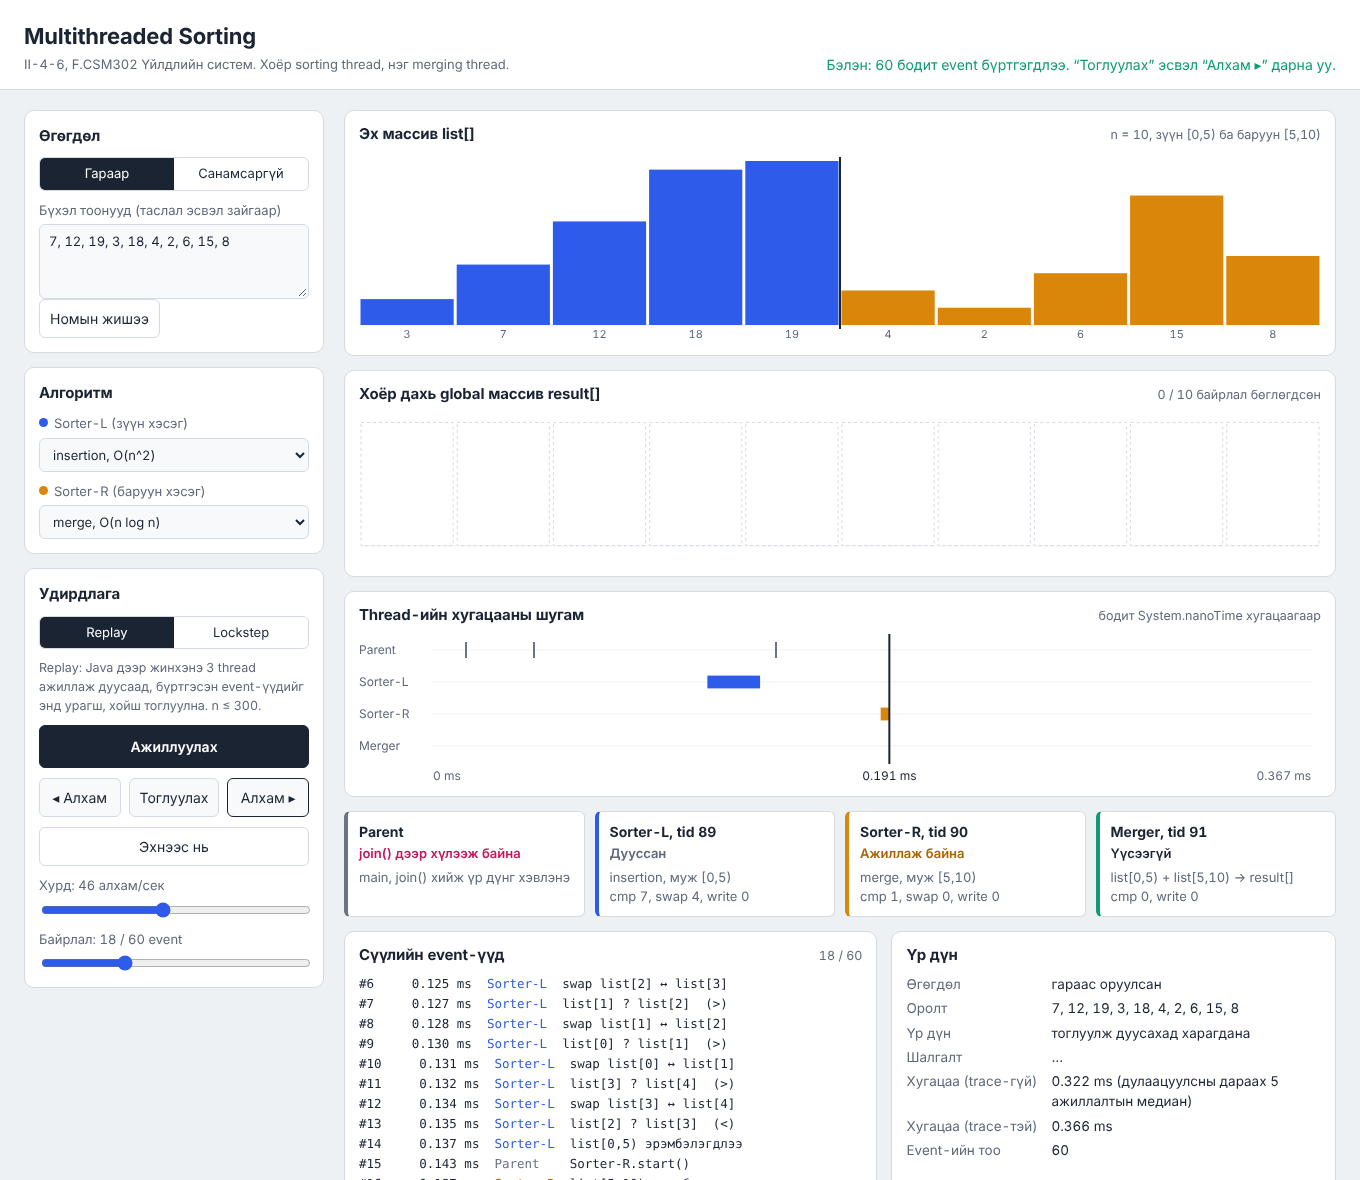
\includegraphics[width=\linewidth]{02-replay-sorting.png}
\caption{Sorter-L хэсгээ эрэмбэлж дууссан, Sorter-R ажиллаж байна}
\end{subfigure}\hfill
\begin{subfigure}{0.49\linewidth}\centering
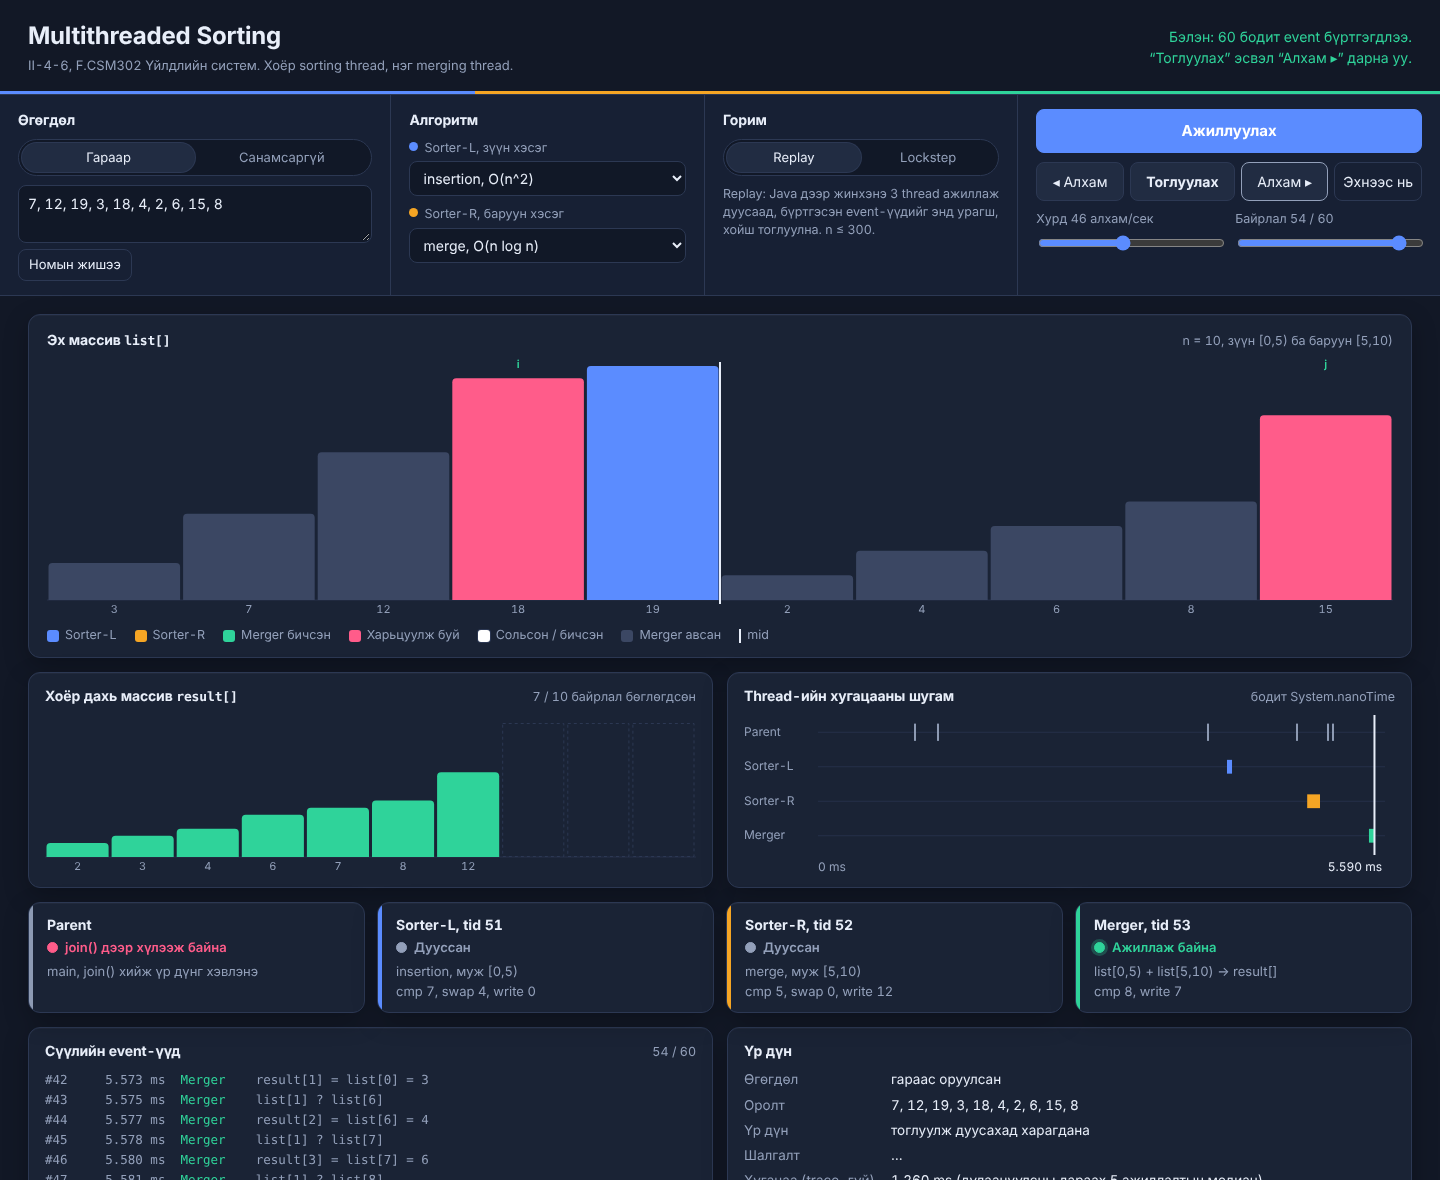
\includegraphics[width=\linewidth]{03-replay-merge.png}
\caption{Merger \code{result[]} руу нэгтгэж байна}
\end{subfigure}
\caption{Replay горим, номын жишээ}\label{fig:ui}
\end{figure}

\section{Replay ба Lockstep горим}
\textbf{Replay} горимд сервер бодит 3 thread-ийг ажиллуулж, бүх event-ийг хөтөч рүү буцаана. Хөтөч эхний $k$
event-ийг эх жагсаалт дээр хэрэглэж дурын алхамд очих тул урагш, хойш явах боломжтой. Мөн trace-гүй ажиллалтын
хугацааг тусад нь харуулна.

\textbf{Lockstep} горимд thread-үүд амьд хэвээр байж, үйлдэл бүрийн өмнө Semaphore дээр зогсоно. “Алхам” бүр
серверт нэг permit өгч, шинэ event-үүд болон thread бүрийн \code{Thread.getState()}-ийг авна (Зураг~\ref{fig:ui-lockstep}).
Бодит thread-ийг буцааж болохгүй тул энэ горимд хойш алхах боломжгүй. Хугацааны тэмдэглэгээ нь хэрэглэгчийн товч
дарах хоорондын хугацааг агуулдаг тул хурд хэмжихэд Replay горимыг ашиглана.

\begin{figure}[H]
\centering
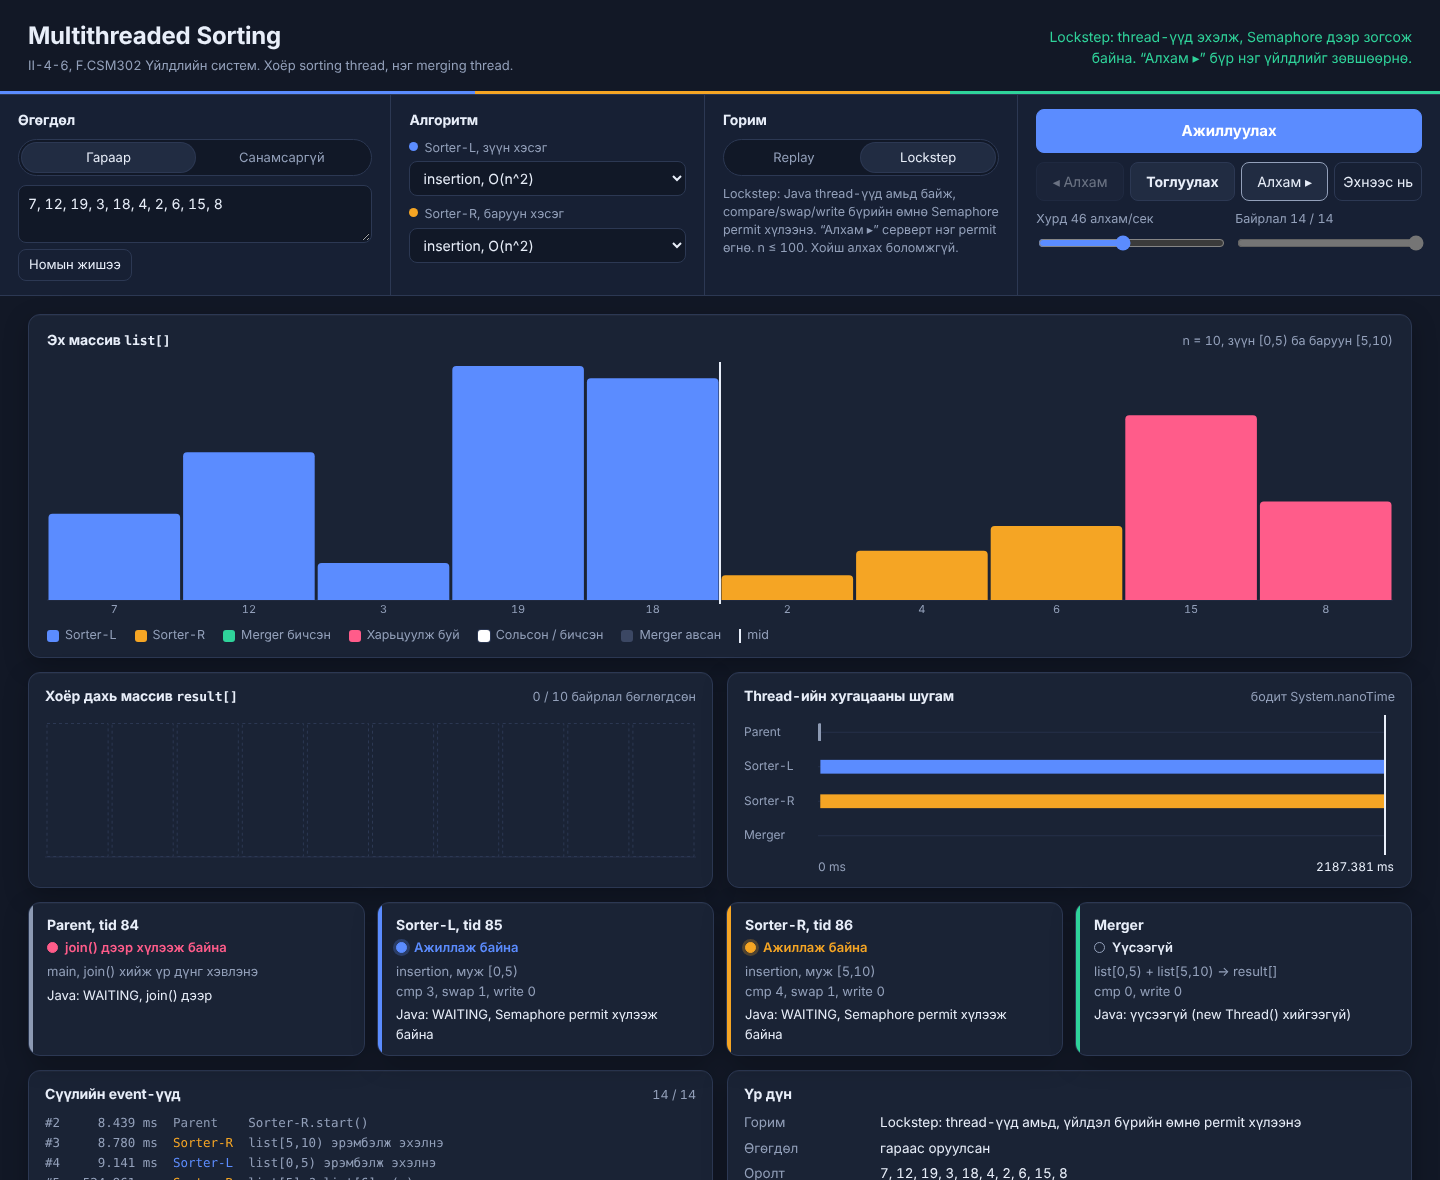
\includegraphics[width=0.72\linewidth]{06-lockstep.png}
\caption{Lockstep: хоёр sorter Semaphore дээр \code{WAITING}, parent \code{join()} дээр \code{WAITING}}\label{fig:ui-lockstep}
\end{figure}
